%% LyX 2.1.4 created this file.  For more info, see http://www.lyx.org/.
%% Do not edit unless you really know what you are doing.
\documentclass[english]{article}
\usepackage[T1]{fontenc}
\usepackage[latin9]{inputenc}
\usepackage{geometry}
\geometry{verbose,tmargin=1in,bmargin=1in,lmargin=1in,rmargin=1in,headheight=1in,headsep=1in,footskip=0.5in}
\usepackage{babel}
\usepackage{graphicx}
\usepackage{algorithm}
\usepackage{algpseudocode}
\usepackage{pifont}
\usepackage[parfill]{parskip}
\newif\ifdraft
\drafttrue
\ifdraft
\usepackage{xcolor}
\definecolor{ocolor}{rgb}{1,0,0.4}
\newcommand{\onote}[1]{ {\textcolor{ocolor} { (***Ole: #1) }}}
\newcommand{\terminology}[1]{ {\textcolor{red} {(Terminology used: \textbf{#1}) }}}
\newcommand{\owave}[1]{ {\cyanuwave{#1}}}
\newcommand{\jwave}[1]{ {\reduwave{#1}}}
\newcommand{\alwave}[1]{ {\blueuwave{#1}}}
\newcommand{\jhanote}[1]{ {\textcolor{red} { ***shantenu: #1 }}}
\newcommand{\alnote}[1]{ {\textcolor{blue} { ***andreL: #1 }}}
\newcommand{\amnote}[1]{ {\textcolor{blue} { ***andreM: #1 }}}
\newcommand{\smnote}[1]{ {\textcolor{brown} { ***sharath: #1 }}}
\newcommand{\pmnote}[1]{ {\textcolor{brown} { ***Pradeep: #1 }}}
\newcommand{\msnote}[1]{ {\textcolor{cyan} { ***mark: #1 }}}
\newcommand{\mrnote}[1]{ {\textcolor{purple} { ***melissa: #1 }}}
\definecolor{orange}{rgb}{1,.5,0}
\newcommand{\aznote}[1]{ {\textcolor{orange} { ***ashley: #1 }}}
\definecolor{dandelion}{cmyk}{0,0.29,0.84,0}
\newcommand{\mtnote}[1]{ {\textcolor{dandelion} { ***matteo: #1 }}}
\newcommand{\gpnote}[1]{{\textcolor{green} {***giannis: #1}}}
\newcommand{\note}[1]{ {\textcolor{magenta} { ***Note: #1 }}}
\else
\newcommand{\onote}[1]{}
\newcommand{\terminology}[1]{}
\newcommand{\owave}[1]{#1}
\newcommand{\jwave}[1]{#1}
\newcommand{\alnote}[1]{}
\newcommand{\amnote}[1]{}
\newcommand{\athotanote}[1]{}
\newcommand{\smnote}[1]{}
\newcommand{\pmnote}[1]{}
\newcommand{\jhanote}[1]{}
\newcommand{\msnote}[1]{}
\newcommand{\mrnote}[1]{}
\newcommand{\aznote}[1]{}
\newcommand{\mtnote}[1]{}
\newcommand{\note}[1]{}
\fi
\begin{document}

\title{Experiments Report}

\maketitle

\begin{abstract}
This report will include the discussion for the experiments. The experiments section will have
data plotting and an initial analysis (model and discussion) based on the developed understanding. 
A Q \& A subsection will follow after the discussion. I will add questions there that still need answering.
It would be nice if others contributed with questions!
\end{abstract}

%\begin{itemize}
%	\item
%	\begin{itemize}
%		\item
%		\item
%		\item 
%		\item 
%		\item 
%		\item 
%		\item
%\end{itemize}


%\begnn{table}[t]
%\centering
%\begin{tabular}{|p{1.6cm}|p{1.6cm}|p{1.6cm}|p{1.6cm}|} \hline
%Property 				  &CPPTraj (RMSD) &Hausdorff Distance &Leaflet Finder\\ \hline
%Single Data Scan      	  &		   &                        & \\ \hline
%Iterative      			  &No 	   &No     &Connected Components \\ \hline5
%
%All-Pairs      			  &No      &Yes          &Pairwise Distance  \\ \hline
%Intermediate Data/Shuffle &Medium  &No Shuffling       & \\ \hline
%Output Data Volume        &Low	   &Low        & \\ \hline
%\end{tabular}
%\caption{Advanced Analytics Application Characteristics}
%\end{table}

%\begin{figure}[t]
%  \includegraphics[width=.45\textwidth]{figures/CPPTrajExecutionSchematicSingleTrajectory.jpg}\quad
%  \caption{}
%  \label{fig:}
%\end{figure}

\section*{CPPTraj RMSD}
The data reported are CPPTraj comparing experiments between Vanilla (MPI) execution and the task parallel execution of CPPTraj via RADICAL-Pilot. The experiments setup is the following:

\begin{itemize}
\item RMSD over 160000 frames as a single trajectory and as an ensemble of 2 trajectories that contain 80000 frames each. (105GB filesize)
\item RMSD over 320000 frames as a single trajectory and as an ensemble of 4 trajectories that contain 80000 frames each. (209GB filesize)
\item RMSD over 640000 frames as a single trajectory and as an ensemble of 8 trajectories that contain 80000 frames each. (418GB filesize)
\end{itemize}

The configuration was from a core per 80000 trajectories up to a node per 80000 frames. All experiments were done on Stampede.

\begin{figure}[H]
\centering
  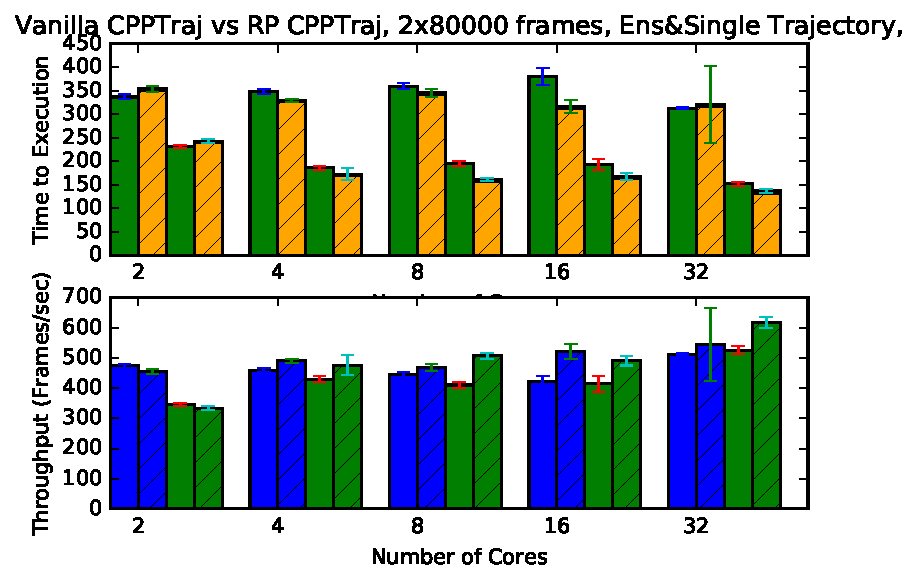
\includegraphics[scale=.70]{cpptraj/cpptrajcomparison_160Kframes.pdf}
  \caption{Time to Execution and Throughput comparison between different ways of executing the same 
  CPPTraj analysis. There are in total 160K frames organized as a single trajectory file for the 
  Single trajectory case and as an ensemble of 2 trajectories for the ensemble case}
  \label{fig:cpptrajcomparison_160Kframes}
\end{figure}

\begin{figure}[H]
\centering
  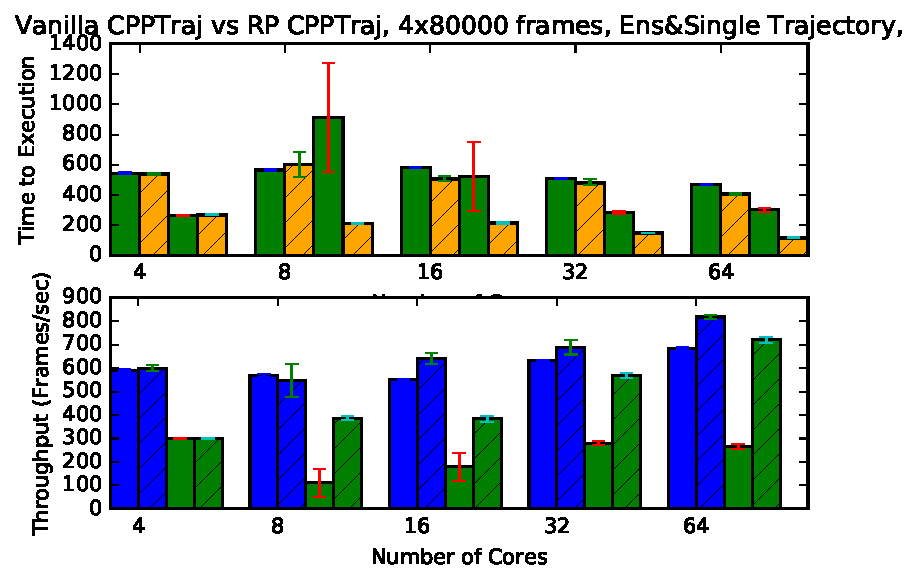
\includegraphics[scale=.70]{cpptraj/cpptrajcomparison_320Kframes.pdf}
  \caption{Time to Execution and Throughput comparison between different ways of executing the same 
  CPPTraj analysis. There are in total 320K frames organized as a single trajectory file for the 
  Single trajectory case and as an ensemble of 4 trajectories for the ensemble case.}
  \label{fig:cpptrajcomparison_320Kframes}
\end{figure}

\begin{figure}[H]
\centering
  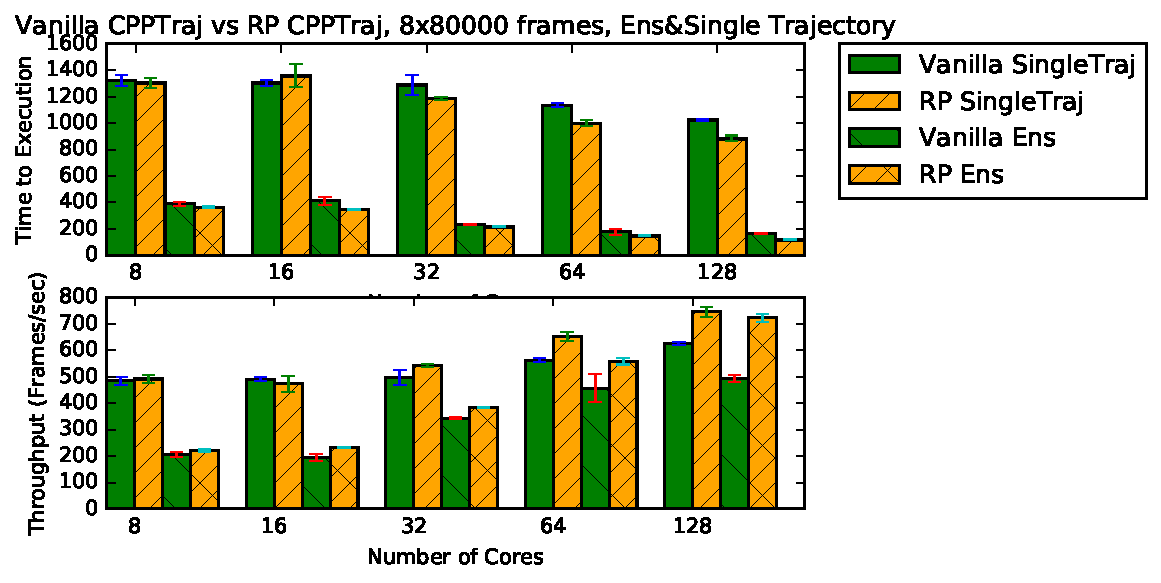
\includegraphics[scale=.70]{cpptraj/cpptrajcomparison_640Kframes.pdf}
  \caption{Time to Execution and Throughput comparison between different ways of executing the same 
  CPPTraj analysis. There are in total 640K frames organized as a single trajectory file for the 
  Single trajectory case and as an ensemble of 8 trajectories for the ensemble case.}
  \label{fig:cpptrajcomparison_640Kframes}
\end{figure}

The top subplot show the Execution time for Vanilla and RADICAL-Pilot. The bottom
subplot shows the Average Throughput. In all figures  the order of the bars is from 
right to left:
\begin{itemize}
\item[1] Single Trajectory Vanilla, 
\item[2] RP-CPPTraj single trajectory,
\item[3] CPPTraj Vanilla Ensemble and 
\item[4] RP-CPPTraj Ensemble
\end{itemize}  

One important note to make, is that as the core count increases, the MPI implementation does not scale in 
ensemble case as the task level parallel for the 320K, Figure \ref{fig:cpptrajcomparison_320Kframes}, and 
640K frames, Figure \ref{fig:cpptrajcomparison_640Kframes}. The main difference between those two is that 
the CPPTraj execution via RADICAL-Pilot introduces a small delay between the launching of each CPPTraj 
process. I believe that this delay reduces the strain CPPTraj's MPI implementation puts to the filesystem 
and the data are read faster. In the next set of experiments with RMSD, I want to find the filesize, or 
better the system size, where the MPI implementation cannot scale anymore and the task level parallel 
can.

The reason behind the above statement is the fact that throughput remains relatively stable. 
Throughput, here measured as frames per second, is the amount of computed data per time unit. We 
can say it is the computation velocity. Throughput is a function of input rate and the number
of computing blocks. By computating blocks, I mean a self contained element that takes an input, does 
some sort of processing on the input and gives an output. In this case,it can either be a MPI process 
or a task.

Assuming that the input rate, throughin, is infinite and it can feed continuously and steadily any number of 
computing blocks, the throughput will increase linearly as we increase the number of computing blocks.
Say that such a block can process $N$ inputs per time unit. Adding a second computing block $2N$ 
inputs per time unit can now be processed. Thus, with $K$ computing blocks the throughput is $KN$ inputs 
per time unit. It is now established how throughput changes when the computation blocks vary and the input rate
is large enough to accomodate any number of them. 

Assume now that the input rate is finite to a maximum of $M$ inputs per time unit. In case $M < N$, throughput
is dectated by the input rate. In case $M \geq N$, throughput will increase linearly as long as the number
of computing blocks is less or equal to $\lfloor\frac{M}{N}\rfloor$. When the number of computing blocks,
becomes larger than the previous number, throuput flats to a rate equal to the rate in which the input is produced.

The question that needs to be answered now is what is the rate that CPPTraj reads in data. The experiments will read
the file and do nothing else. 

\section*{Hausdorff Distance}

The data reported here are comparing the Hausdorff Distance calculation via a RADICAL-Pilot and a 
Spark implementation. Both use the same implementation for the main function and both use parallel
read. The experiments were executed over 192 trajectories of CA atoms on Comet. Figure 
\ref{fig:HausdorffMeanTaskBreakDownPr} show the mean time to execution for all three cases of 
trajectory size for the CA atoms. 

\begin{figure}[H]
\centering
  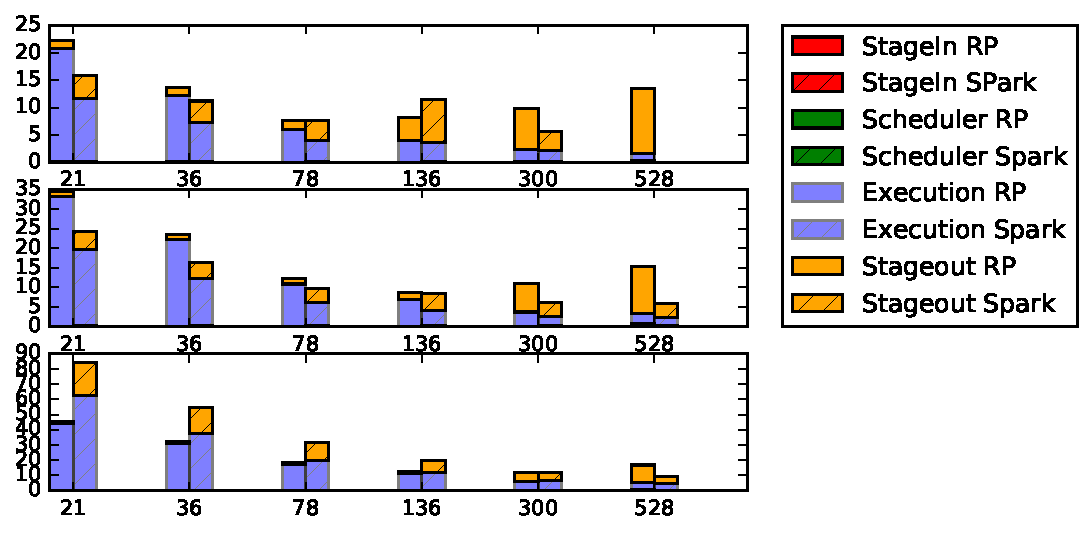
\includegraphics[scale=.70]{Hausdorff/MeanTaskBreakDownPr.pdf}
  \caption{Time to Execution Hausdorff Distance. From top to bottom Short trajectory, Medium 
           Trajectory, Long Trajectory}
  \label{fig:HausdorffMeanTaskBreakDownPr}
\end{figure}

Figures \ref{fig:DetailedMeanTaskBreakDownShort},\ref{fig:DetailedMeanTaskBreakDownMed} and 
\ref{fig:DetailedMeanTaskBreakDownLong} show in more detail how the execution between the two 
frameworks differ. Two main differences is that RADICAL-Pilot spends more time to stage in and 
stage out data to and from a task, where Spark is more expensive in scheduling tasks.

\begin{figure}[H]
\centering
  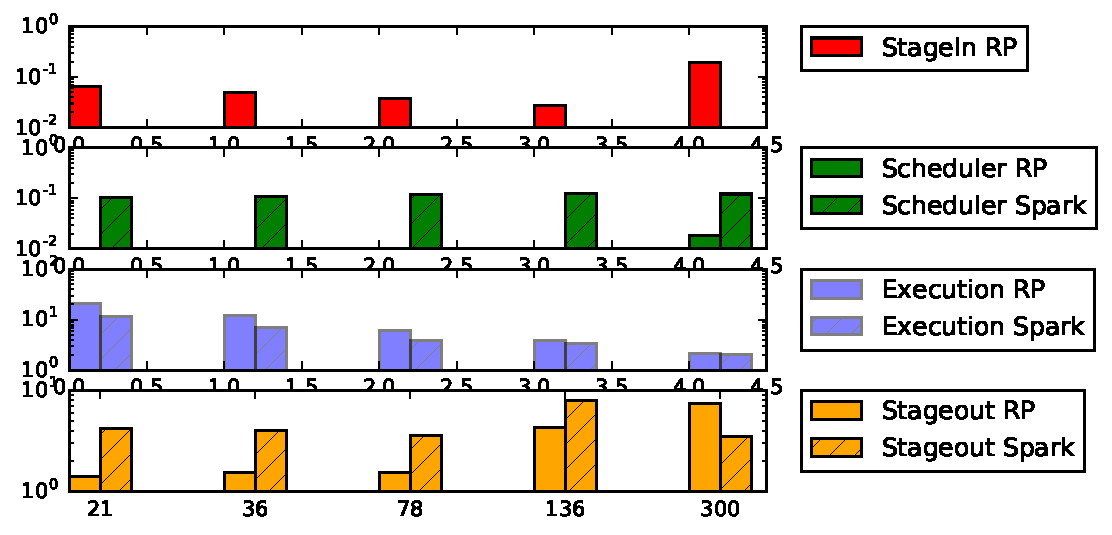
\includegraphics[scale=.70]{Hausdorff/DetailedMeanTaskBreakDownShortPr.pdf}
  \caption{Execution break down between RADICAL-Pilot and Spark execution. The Y axis represents 
  the time spent in each part and the X axis the number of core. This is short trajectory size}
  \label{fig:DetailedMeanTaskBreakDownShort}
\end{figure}

\begin{figure}[H]
\centering
  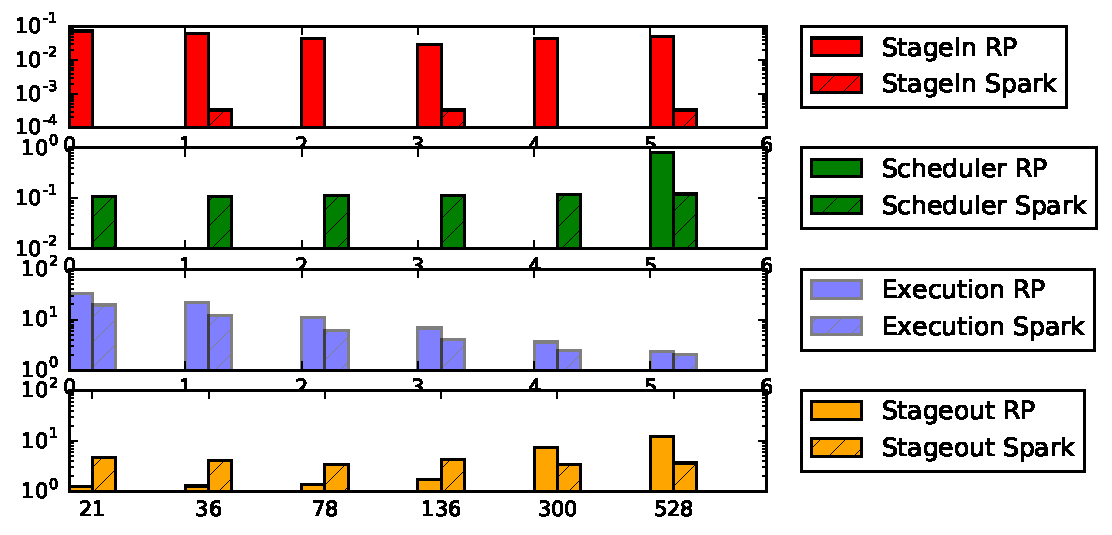
\includegraphics[scale=.70]{Hausdorff/DetailedMeanTaskBreakDownMedPr.pdf}
  \caption{Execution break down between RADICAL-Pilot and Spark execution. The Y axis represents 
  the time spent in each part and the X axis the number of core. This is medium trajectory size}
  \label{fig:DetailedMeanTaskBreakDownMed}
\end{figure}

\begin{figure}[H]
\centering
  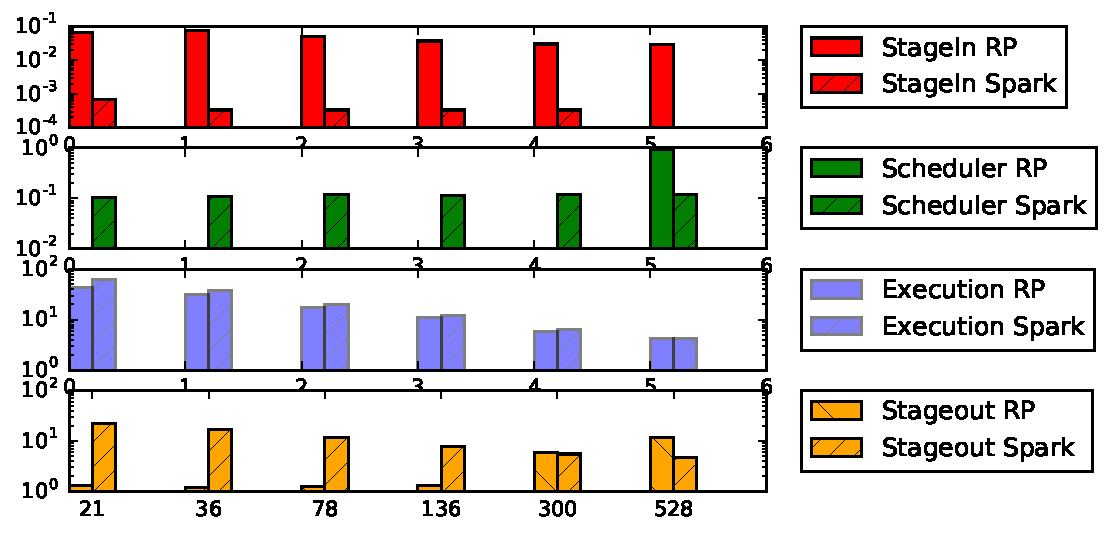
\includegraphics[scale=.70]{Hausdorff/DetailedMeanTaskBreakDownLongPr.pdf}
  \caption{Execution break down between RADICAL-Pilot and Spark execution. The Y axis represents 
  the time spent in each part and the X axis the number of core. This is Long trajectory size}
  \label{fig:DetailedMeanTaskBreakDownLong}
\end{figure}

Extra experiments were executed with the following configuration on Comet:
\begin{itemize}
\item Number of trajectories is 128
\item Number of atoms 214 and frames 102. Trajectory sizes are Short, Medium and Long. This is
      equivalent to 214 atoms per frame, 428 and 856 respectively.
\item The whole matrix was calculated
\item Core count: 16, 64, 256 and 1024
\item Execution was done with RADICAL-Pilot and Pilot-Spark.
\end{itemize}

The following figures show that comparison.

\begin{figure}[H]
\centering
  \includegraphics[scale=.45]{Hausdorff/MeanTaskBreakDownPower2.pdf}
  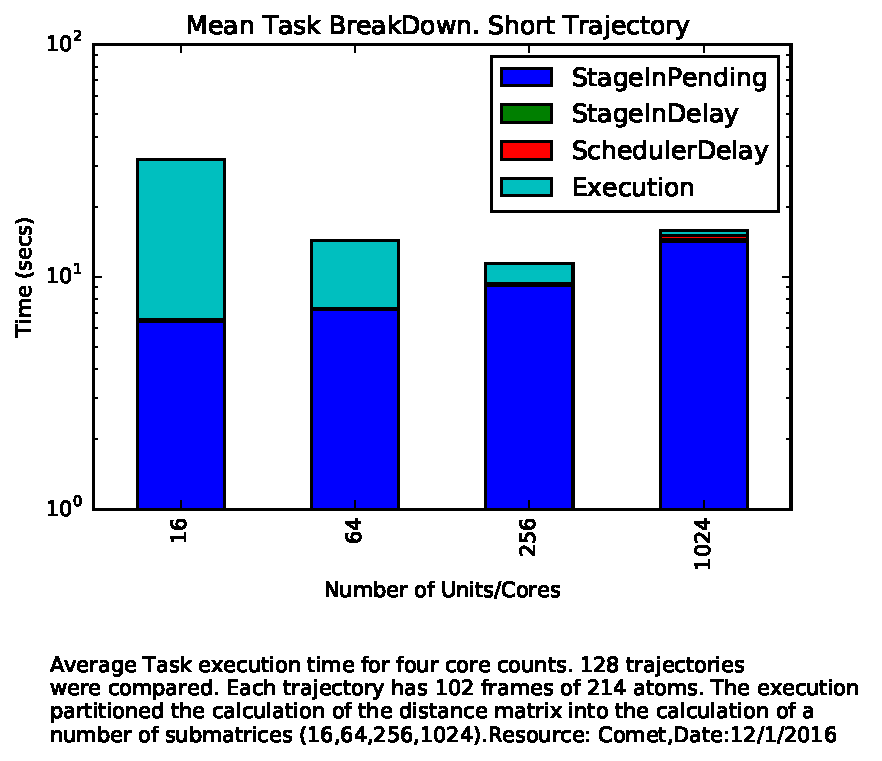
\includegraphics[scale=.45]{Hausdorff/LogMeanTaskBreakDownPower2Short.pdf}
  \label{fig:MeanTaskBreakDownPower2Short}
\end{figure}

\begin{figure}[H]
\centering
  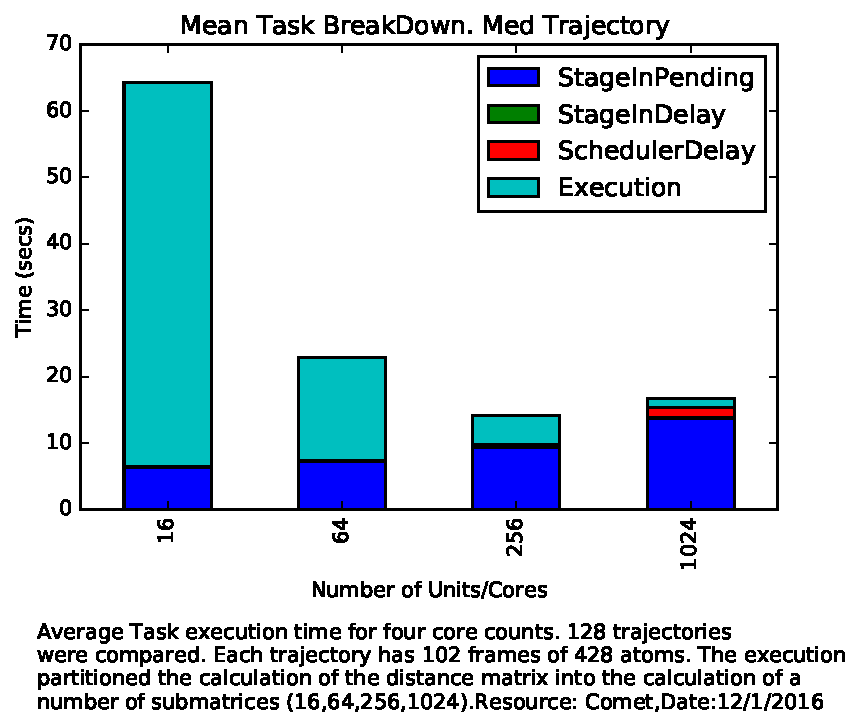
\includegraphics[scale=.45]{Hausdorff/MeanTaskBreakDownPower2Med.pdf}
  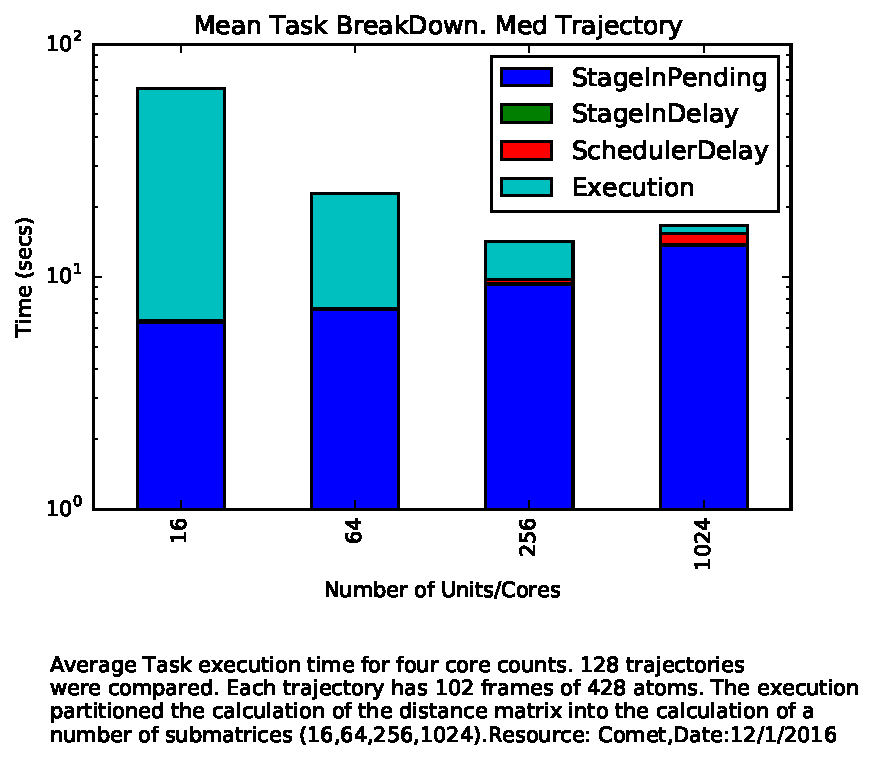
\includegraphics[scale=.45]{Hausdorff/LogMeanTaskBreakDownPower2Med.pdf}
  \label{fig:MeanTaskBreakDownPower2Med}
\end{figure}

\begin{figure}[H]
\centering
  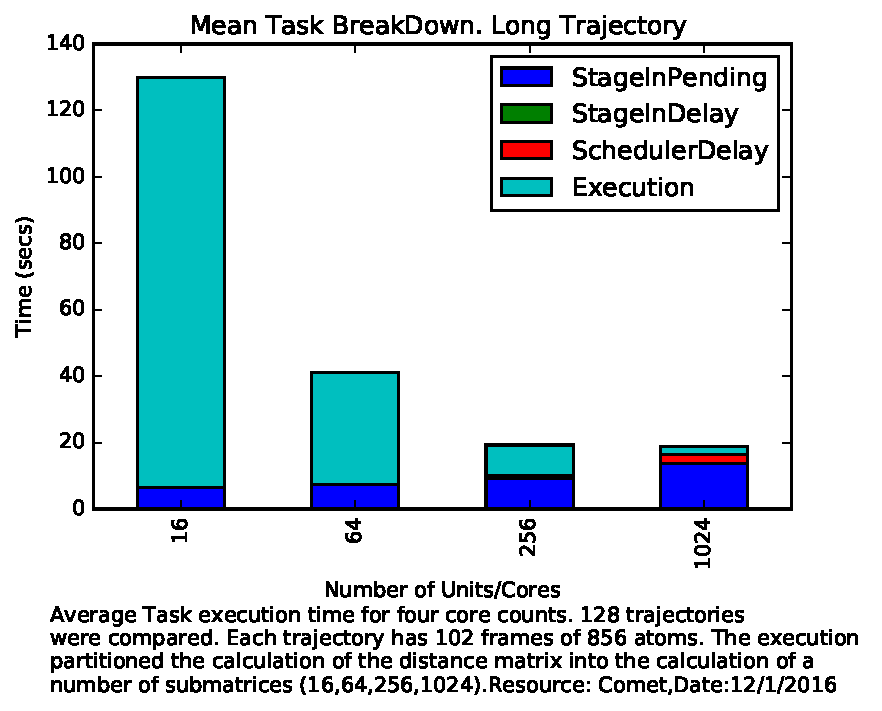
\includegraphics[scale=.45]{Hausdorff/MeanTaskBreakDownPower2Long.pdf}
  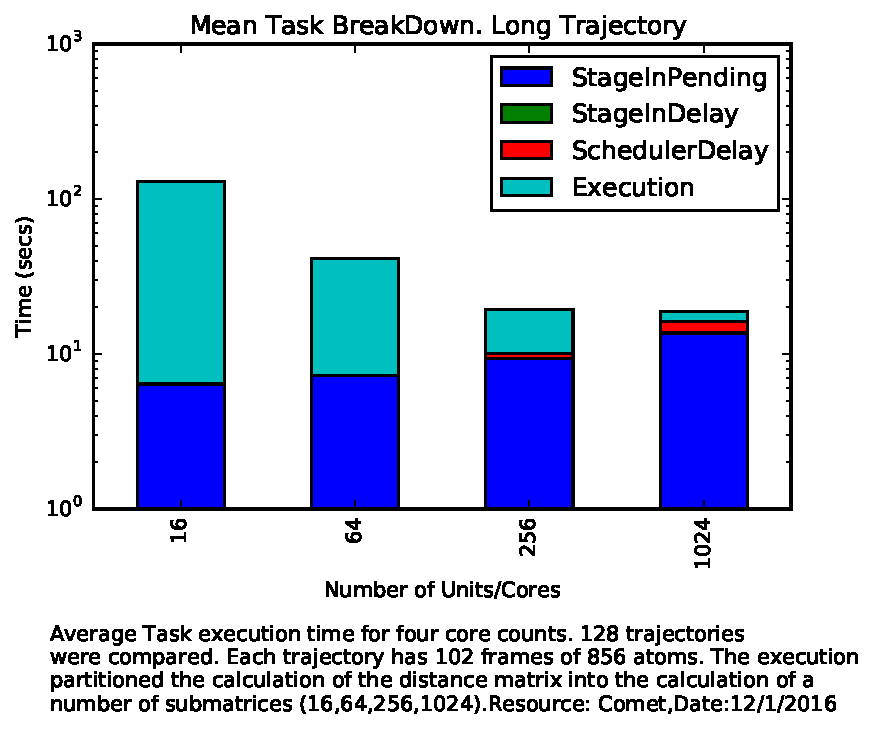
\includegraphics[scale=.45]{Hausdorff/LogMeanTaskBreakDownPower2Long.pdf}
  \label{fig:MeanTaskBreakDownPower2Long}
\end{figure}

\subsection*{Useful Definitions [Updated*]}
\begin{itemize}
\item $N_{Tr}$: Number of Trajectories per task
\item $N_A$: Number of atoms in a frame.
\item $N_F$: Number of frames per trajectory. All trajectory files have the same number of 
frames, 102.
\item $N_T$: Number of tasks
\item $\alpha$: the coefficient of Staging In
\item $\beta$: the coefficient of the Scheduling delay
\item $\gamma$: the coefficient of the Execution
\item $\delta$: the coefficient of the Staging Out
\end{itemize}

\subsection*{Analysis}
The execution model can be easily broken to different parts.  First part of the model is data 
StageIn. In case of RADICAL-Pilot StageIn is rather easy to undeerstand. In case of Spark, I 
consider as StageIn the part of the code that is written before partitioning the data. Second part 
is the time need to schedule a task. Third is the actual execution of the task, which can be broken 
further more to read, exec and write. Finally, the last part of the model is the time necessary to 
stage out the data. In case of RADICAL-Pilot it is easy to understand. In Spark, I consider as the 
time needed from the time that all tasks have returned their data until the end of the script.

\gpnote{Why is the need for every parameter?}

Essentially, the model will look like:

$$T=\alpha(N_I)+\beta N_T+\gamma Y+\delta\Big{(}N_O S_O + \frac{k(k+1)}{2}\Big{)}$$

$Y$ is the tme of the execution of the task.
\subsubsection*{Task Execution Analysis}
That is dependent to the number of trajectories being processed and the number of points in each 
trajectory. Let $T_N$ be the number of trajectories per task and $T_S$ the size of each trajectory, 
i.e. the number of points.Thus, the above execution time can be

$$Y = \Big{O}((N_Tr N_F N_A)^2)$$

Let $dH$ be the time to calculate the Hausdorff distance between two trajectories. The following 
algorithm describes it in pseudocode. The description will help the following analysis:

\begin{algorithm}
\begin{algorithmic}[1]
\Procedure{HausdorffDistance}{$T_1,T_2$}\Comment{$T_1$ and $T_2$ are a set of 3D points}
\For{\forall $t_1$ in $T_1$}
\For{\forall$t_2$ in $T_2$}
\State \texttt{Append in $D_1$ calculated d($t_1, t_2$)}
\EndFor
\State\texttt{$D_t_1$ append max($D_1$)}
\EndFor
\State $N_1$ = min($D_t_1$)
\For{\forall $t_2$ in $T_2$}
\For{\forall$t_1$ in $T_1$}
\State \texttt{Append in $D_2$ calculated d($t_2, t_1$)}
\EndFor
\State\texttt{$D_t_2$ append max($D_2$)}
\EndFor
\State $N_2$ = min($D_t_2$)
\State \textbf{return} max($N_1$,$N_2$)
\EndProcedure
\end{algorithmic}
\end{algorithm}

Thus, the complexity of $dH$ is

$$dH =\mathcal{O}({T_S}^2) + T_S \mathcal{O}(T_S) + \mathcal{O}({T_S}^2) + T_S \mathcal{O}(T_S)$$

\subsection*{RP Fitting}
Before solving any system, I will add some assumptions that will try to simplify the 
model as well as better understand how the scheduler and data stage in overheads 
affect the execution.

\begin{itemize}
\item RADICAL-Pilot's staging output does not affect the execution pattern of the
tasks. All tasks are executed in parallel and there is no data movement from the 
executing resource to the client. Also, there is no continuation in the execution
since only one pass is done over the data.
\item Any delay between the moment a Compute Unit goes to the Executing state and starts execute as well 
as the delay from the moment it returns until it moves to the next stage, are assumed as part of the 
execution time of the task.
\item Parameter $\gamma$ is set to 1 in this case, because the timing parameters for the execution are
captured inside $Y$.
\end{itemize}

\gpnote{What is $x^2$ value? What is the goodness of the values? What is the error in all these?}

[Update]
The execution time of the tasks depend on the number of trajectory files that it gets, the number
frames per trajectory and the number of atoms. The number of atoms affects the exeution time linearly,
the number of frames and the number of trajectories affect in a squared fashion.

Thus $T_{Ex}(N_{Tr},N_A,N_F) = e_1 N_{Tr}^{2} N_{F}^{2} N_A + e_2$

After appling the least square method the values found for $e_1$ and $e_2$ are:
$$e_1=1.33271794e-08 \quad e_2=8.09404416e-02$$

The $\chi^2$ test was applied to the following points:

\begin{table}[H]
\centering
\begin{tabular}{|c|c|c|c|c|} \hline
Trajectories&Frames&Atoms& Observed Time &Predicted Time \\ \hline
32&102&214&25.46786774&30.46545617 \\ \hline
16&102&214&7.00346226&7.67706937 \\ \hline
 8&102&214&2.0758777&1.97997267  \\ \hline
 4&102&214&0.76485454&0.5556985 \\ \hline

32&102&418&57.81401424&60.84997191 \\ \hline
16&102&418&15.59695303&15.27319831 \\ \hline
 8&102&418&4.39942563&3.87900491  \\ \hline
 4&102&418&1.3047394&1.03045656 \\ \hline

32&102&856&123.41059877&121.61900337 \\ \hline
16&102&856&33.88301111&30.46545617 \\ \hline
 8&102&856&9.16800458&7.67706937  \\ \hline
 4&102&856&2.56352096&1.97997267 \\ \hline
\end{tabular}
\end{table}

The tested null hypothesis is the observed values belong to the predicted distribution

The $\chi^2$ is calculated with the following formula:

$$ \chi^2 = \sum^{12}_{1} \frac{(O_i - P_i)^2}{P_i}$$

The $\chi^2$ value is $2.13474849056$. This value is smaller than the $\chi^2_0.05$ for $11$ 
degress of freedom, thus we cannot reject the null hypothesis for the $0.05$ significance 
level.

The Last Unit arrival time is considered as the time the last CU entered the State 
AgentStagingInput where input staging start to be executed.

The Least Squares Fit was done over the points obtained for 16, 64, 256 and 1024 CUs.
The line that was obtained is the following

$$T_{A}(N_T) = 0.01313076 N_T + 7.66860076 $$

\subsection*{Spark Fitting}

The Spark execution model requires one extra term. That term is shows the time that is needed to
for Spark to launch its executors. An executor is the process responsibe to execute the tasks. An 
assumption that is made is the fact that stagein in the Spark execution does not significantly 
change the execution time since it creates an RDD with the paths where the file are. So,
the model will be 

$$T=\beta\frac{k(k+1)}{2}+ Y +\delta\Big{(}N_O S_O + \frac{k(k+1)}{2}\Big{)}+\epsilon W$$

where $W$ is the number of worker nodes.

\gpnote{TODO: Solve the system}

\end{document}
